% !TeX root = ../main.tex
% Add the above to each chapter to make compiling the PDF easier in some editors.

\chapter{Evaluation}\label{chapter:evaluation}

\section{Running Benchmarks}

When implementing the workloads for our benchmarks, we noticed that using WebAssembly as of now imposes many constraints. Since we are not targeting a browser platform, which offers a wide variety of APIs meant to handle system calls, this means that code targeting WASM on the ESP32 can not make use of APIs available in the browser environment such as memory allocation. This is where WASI comes into play, as mentioned in \ref{sec:b_wasm}, WASI aims to solve the problem of interfacing with the system from WASM code by providing a standardized interface. Once WASI is supported by the runtime, writing code for it will be much more straightforward.

In order to run the test, we had to compile the C++ test code into WASM bytecode. An established tool for this is the emscripten compiler. After using this for the initial tests, though, we noticed problems, since it is meant for compiling WASM that will run in the browser. This leads to modules that expect all the available functions of the browser environment since we are running the tests on an embedded device; those functions are not available to us.

\begin{sloppypar}
Because emscripten is meant for use in browsers after compilation, we switched to the \lstinline{wasmc++} compiler, which is part of wasienv, a toolchain for compiling C into WebAssembly \autocite{noauthor_wasienvwasienv_2020}. This project provides a couple of utilities to compile C code into WASM modules. \lstinline{wasmc++} wraps clang++ with the correct configuration for WebAssembly already applied and makes compiling very easy. For our tests, the code was compiled by running \lstinline{wasmc++ -Os -Wl,--strip-all -nostdlib wasm/test.cpp -o wasm/test.cpp.wasm}.
\end{sloppypar}

\begin{sloppypar}
Lastly, the WASM3 runtime expects the bytecode to be loaded into an array. In Linux, the \lstinline{xxd} utility is exactly what is needed to achieve that. After compilation, the WASM code can be converted into a C++ header file by running \lstinline{xxd -i wasm/test.cpp.wasm > main/test.wasm.h}. After these steps, we are able to run our tests just as planned.
\end{sloppypar}

After designing tests as described in \ref{subsec:testing_setup}, we ran all of them on the ESP32 to report times. In general, the tests showed a significant slowdown in execution speed when running the workloads in a WebAssembly context compared to running them compiled natively. For all tests, we could observe the variance of the measured time is very low; this is to be expected since the tests ran without any other load on the MCU and the deterministic nature of FreeRTOS, as mentioned in section \ref{subsec:freertos}.

It is important to mention when looking at the result of these tests that WASM3 heavily relies on tail call elimination, which currently is not performed by the ESP32 compiler. This leads to excessive use of the native stack and lower performance. Collaborators and authors of WASM3 are currently exploring solutions that would make the runtime faster and more efficient on the platform soon \autocite{grokhotkov_esp32-idf_nodate}.

\subsection{Recursive calls}\label{subsec:eval_recursive}

Calling functions is an integral capability of any application, so this is the first test to compare WASM with the native execution of our code. We are using the test described in \ref{subsec:m_test_recursive}. This test has almost no instructions but produces many function calls that could be troubling to handle for the runtime.

Even though most applications on an MCU might not run recursive calculations, this test does show the cost of calling many functions. Table \ref{tab:times_recursive} shows some of the measured times. It is apparent from the numbers that running the code in the interpreter takes about 41x longer than the native execution.

As seen in the WASM code of listing \ref{lst:recursive_wat}, it is straightforward but requires the runtime to manage the execution of the same functions many times over. Compared to some of the following tests, 41x is not a very high slowdown.

To see if both the runtime and native execution behave similarly for different inputs, we ran the test multiple times. Figure \ref{fig:times_recursive} shows the change in execution time for rising input. As expected, the execution time grows exponentially, but the runtime and native execution maintain their 41x difference in speed.

\begin{table}[h]
    \begin{tabular}{l c c}
        Run & WASM Execution & Native Exectuion \\
        10  & 41766          & 1000             \\
        11  & 41767          & 1000             \\
        12  & 41766          & 1000             \\
        13  & 41767          & 1000             \\
        14  & 41766          & 1000             \\
        15  & 41767          & 1000             \\
        16  & 41766          & 1000             \\
        17  & 41766          & 1000             \\
    \end{tabular}
    \caption{Exerpt of the measured times for recursive calls}
    \label{tab:times_recursive}
\end{table}

\begin{figure}[h]
    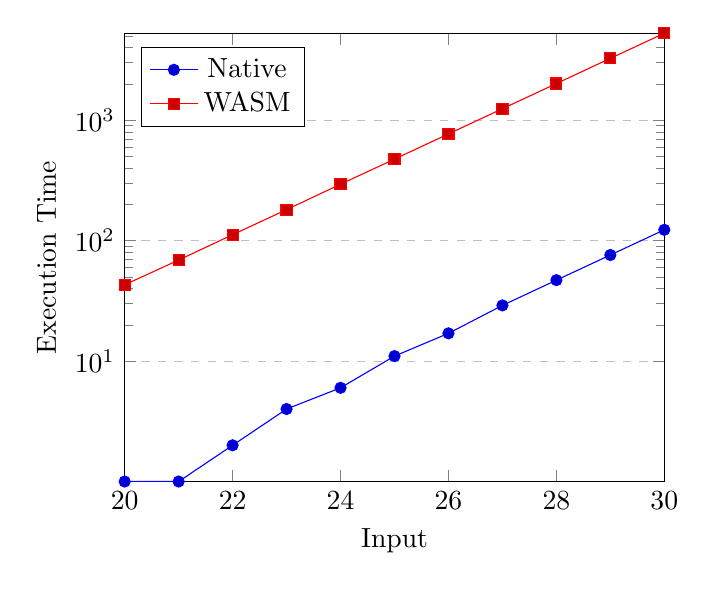
\begin{tikzpicture}
        \begin{axis}[
            xlabel={Input},
            ylabel={Execution Time},
            xmin=20, xmax=30,
            ymin=1, ymax=5274,
            ymode=log,
            xtick={20,22,24,26,28,30},
            ytick={0,10,100,1000,10000},
            legend pos=north west,
            ymajorgrids=true,
            grid style=dashed,
        ]
            \addplot coordinates {(20,1)(21,1)(22,2)(23,4)(24,6)(25,11)(26,17)(27,29)(28,47)(29,76)(30,123)};
            \addplot coordinates {(20,43)(21,69)(22,112)(23,181)(24,294)(25,475)(26,769)(27,1245)(28,2014)(29,3260)(30,5274)};
            
            \legend{Native, WASM}
        \end{axis}
    \end{tikzpicture}
    \caption{Recursive call times for different inputs}
    \label{fig:times_recursive}
\end{figure}

\subsection{Swicth statements}

Next, we tested the performance of switch statements in the runtime. The times listed in Table \ref{tab:times_switch} lead to the conclusion, that the native compiler optimized our switch statement very well, effectively skipping over what we tried to test. Otherwise, the native instruction should take a while longer. Since the WASM code never executed more than 100x slower than native code, it would be reasonable to expect a result in the same range for switch statements.

Since there are no values to compare this statement by, we cannot pass judgment on how much of a performance hit switch statements take from being executed in the runtime. It is fair to assume a similar slowdown to the other tests occurs here.

\begin{table} [h]
    \begin{tabular}{l c c}
        Run & WASM Execution & Native Exectuion \\
        24  & 1021           & 0                \\
        25  & 1021           & 0                \\
        26  & 1021           & 0                \\
        27  & 1021           & 0                \\
        28  & 1021           & 0                \\
        29  & 1021           & 0                \\
        30  & 1021           & 0                \\
        31  & 1021           & 0                \\
    \end{tabular}
    \caption{Exerpt of the measured times for switch calls}
    \label{tab:times_switch}
\end{table}

\subsection{Memory access}

Of course, every application requires memory access, so we ran tests that perform linear reads on the memory. The runtime caused a longer execution time of around 33x, as can be seen in the measured times in table \ref{tab:times_memory}. Since WASM is always run in a virtual machine, memory access optimization is not achieved in the source code but instead taken care of by the runtime. In a browser, for example, the WASM memory is a JavaScript ArrayBuffer.

We were not able to directly compare linear memory access with random memory access. However, when running the test meant to assess random access, we saw the performance loss increase to about 73x. This could be caused by several things, such as the generation of pseudo-random numbers in the test code. We can not make a precise determination if random access has any impact on the performance of the WASM code.

\begin{table} [h]
    \begin{tabular}{l c c}
        Run & WASM Execution & Native Exectuion \\
        74  & 1802           & 56               \\
        75  & 1801           & 55               \\
        76  & 1802           & 55               \\
        77  & 1802           & 55               \\
        78  & 1802           & 55               \\
        79  & 1802           & 55               \\
        80  & 1801           & 55               \\
        81  & 1802           & 55               \\
    \end{tabular}
    \caption{Exerpt of the measured times for memory access}
    \label{tab:times_memory}
\end{table}

\subsection{Matrix multiplication}

The matrix multiplication test combines both memory access and calculations and experiences the most significant increase of execution time in any of our tests. As the numbers in table \ref{tab:times_matrix} show, the interpreted code runs more than 90x slower than the natively executed code.

This test does show that more extended calculations and more sophisticated algorithms will take a significant performance hit when being run as WebAssembly. Even in contact with the contributors of the runtime, we were not able to identify specific tasks that are very expensive in the interpreted environment. Nevertheless, as a general rule, it is not advisable to implement large complex workloads in WebAssembly at this point.

\begin{table} [h]
    \begin{tabular}{l c c}
        Run & WASM Execution & Native Exectuion \\
        55  & 26277          & 281              \\
        56  & 26277          & 282              \\
        57  & 26277          & 281              \\
        58  & 26277          & 281              \\
        59  & 26277          & 282              \\
        60  & 26277          & 281              \\
        61  & 26277          & 281              \\
        62  & 26277          & 281              \\
    \end{tabular}
    \caption{Exerpt of the measured times for matrix multiplication}
    \label{tab:times_matrix}
\end{table}

\subsection{Calling of native code}

Of course, not all functionality can be included in the WASM module; especially native platform features will have to make use of functions only available outside of the module. When measuring the performance of calls outside the test-module, we are taking the total time of ten runs. The timings in table \ref{tab:times_native} show that the overhead introduced by the runtime for such a simple test case is relatively small. The interpreted code took less than 10x longer than the native calls.

In a second test, which also returned a value to the WASM module, we did not see an additional increase in execution time, making this the best performing test in our experiments.

\begin{table} [h]
    \begin{tabular}{l c c}
        Run & WASM Execution & Native Exectuion \\
        15  & 33             & 7                \\
        16  & 33             & 8                \\
        17  & 33             & 7                \\
        18  & 32             & 8                \\
        19  & 33             & 8                \\
        20  & 32             & 8                \\
        21  & 33             & 8                \\
        22  & 32             & 7                \\
        23  & 33             & 8                \\
        24  & 32             & 7                \\
        25  & 33             & 8                \\
    \end{tabular}
    \caption{Exerpt of the measured times for external calls}
    \label{tab:times_native}
\end{table}

\subsection{Typescript execution}

Colesely related to \ref{subsec:eval_recursive} is the test case running TypeScript, since it is the same test function and almost the same WASM code being tested. The observed results in table \ref{tab:times_typeScript} are very similar to the times measuren when executing WebAssembly code genrated from C++. Nonetheless, this test shows the exciting potetntial of running languages on the ESP32 that are not natively supported. Also it's interesting to note that, at least for this example, there is no performance loss by using TypeScript instead of C++.

\begin{sloppypar}
    Of course the compilation of TypeScript to WebAssembly requires a different compiler than \lstinline{wasmc++}. We used the \lstinline{asc} compiler that is part of the AssemblyScript toolchain and compiled the TypeScript code by running \lstinline{asc index.ts -b test.wasm --validate -O3z --runtime none --noAssert}. After compilation we followed the same steps as with the other tests to run the comparison.
\end{sloppypar}

\begin{table}[h]
    \begin{tabular}{l c c}
        Run & WASM Execution & Native Exectuion \\
        37  & 41493          & 1000             \\
        38  & 41493          & 1000             \\
        39  & 41493          & 1000             \\
        40  & 41493          & 1000             \\
        41  & 41493          & 1000             \\
        42  & 41493          & 1000             \\
        43  & 41493          & 1000             \\
        44  & 41493          & 1000             \\
        45  & 41493          & 1000             \\
        46  & 41494          & 1000             \\
    \end{tabular}
    \caption{Exerpt of the measured times for TypeScript execution}
    \label{tab:times_typeScript}
\end{table}

\section{Learnings}
\subsection{Drawbacks of WASM execution}
The very obvious drawback of executing WebAssembly on a microcontroller is the performance loss that comes with it. We have shown this with all our tests, and even though the slowdown varies from test to test, code compiled to WASM and executed by an interpreter will run an order of magnitude slower than the same code directly compiled into the main program and executed on the MCUs CPU.

This puts WebAssembly into an unexpected position on embedded devices since it is meant initially to provide better performance. In browsers, WebAssembly made it possible to run adobe lightroom on the web, allows Facebook to compress images before uploading them and Wikipedia to play videos the users' browser does not support \autocite{wagner_webassembly_2017}. However, even though it reaches near-native speeds on browsers, it performs much worse than the current alternative on embedded devices.

It is fair to assume that this performance decrease causes the MCU to consume much more energy in order to make the same computation. For devices running on a battery, this could pose a challenge. Further experiments could be made to quantify the impact of running WASM and also compare it to other energy-consuming tasks such as network IO.

Apart from the impact on the running of program code on the MCU, we also noticed other limitations. The availability of certain expected functionality in WASM is minimal. For example, the use of \lstinline{malloc()} is not possible if compiling code to WASM and running it in our runtime. In web browsers, this functionality is available for import from the environment and implemented such that it can be used as expected. WASM3, however, does not offer any functions for import, and implementing dynamic memory management would be a significant effort.

Since the problem of system access outside the browser is prevalent, a subgroup of the WASM community group is working on specifying a system interface for WASM\autocite{clark_standardizing_2019}. The WebAssembly system interface (WASI) is meant to provide a foundation for developers to build upon when targeting non-browser platforms. Once specified, code compiled for WASI will run in any WASI-compliant runtime, truly enabling WASMs portability.

\subsection{Potential of WebAssembly on embedded devices}

As we demonstrated in our tests, the WebAssembly code is interpreted at runtime; this means that it could also be loaded from the network instead of being included in the code. Dynamically loading code and executing it allows the deployment of new behavior to an MCU without having to perform a flash but rather in the form of an over the air update.

Since WebAssembly support in the browser is excellent already, all the tests we developed can alternatively be run in the browser. This allows embedded developers to test their programs locally in development and be able to make sure everything works as expected even before deploying it to an MCU for the first time. For the ESP32, for example, a browser emulator could be built, which provides all the native functions expected on the platform in JavaScript.

Additionally, we showed in the last test that WebAssembly can open the doors for new languages that are not natively supported on the MCU. In our example, we were able to program the ESP32 by using TypeScript, which usually compiles to JavaScript. However, in our example, we compiled it to WebAssembly and were able to run it on the ESP32. This enables developers without previous to get into embedded programming from their current field of work.

\subsection{Usecase examples on the ESP32}

For embedded use-cases that are CPU bound, WebAssembly could pose a big problem since the performance is much worse than current native execution. Making up for this with multiple devices could be a way of mitigating that problem, but since we have observed a performance loss of close to 100x, that seems like a costly way of overcoming this problem.

Should the most time-consuming things not be calculations and similar tasks, though, but waiting for a slow sensor read or a signal from the outside, the performance loss might not be as significant. Execution time also matters less if the task is performed periodically, and the device has much idle time.

A very promising use-case of WASM is the customization of device behavior. This example is often given and also supported by the results of our tests and relies on the interoperation of the native code with the loaded WASM module. An IoT device could, for example, have an extensive API and allow the user to deploy logic in the form of a WebAssembly module making use of all the API functions. Here, other features of WebAssembly also come into play, such as it is security guarantees, which make it safer to execute unknown code on the device.

\section{Summary}